% main.tex  --  ICDM 2026 submission
% Title: Coverage Is Not Predictive Fidelity: A Split-Landscape Analysis of Data
%        Condensation for Gradient-Boosted Trees

\documentclass[conference]{IEEEtran}

% ============================================================
%  PACKAGES  (order matters — do not reorder)
% ============================================================

% Font encoding — avoids missing OT1/Courier TFM on some TeX Live installs
\usepackage[T1]{fontenc}
\usepackage{lmodern}

% Math
\usepackage{amsmath}
\usepackage{amssymb}
\usepackage{amsfonts}

% Graphics
\usepackage{graphicx}

% Tables
\usepackage{booktabs}
\usepackage{multirow}
\usepackage{array}

% Sub-figures
\usepackage{subcaption}

% Algorithms (algpseudocode for \State, \Require, \Ensure, \Comment, \Return)
\usepackage{algorithm}
\usepackage{algpseudocode}

% Numbers / units
\usepackage{siunitx}
\sisetup{detect-weight=true, mode=text}

% Color
\usepackage{xcolor}

% Structured statement environments
\usepackage{amsthm}
\newtheorem{lemma}{Lemma}
\newtheorem{definition}{Definition}

% Bibliography (IEEE style)
\usepackage{cite}

% TikZ
\usepackage{tikz}
\usetikzlibrary{arrows.meta,positioning,shapes.geometric,calc,fit,backgrounds}

% Hyperlinks (load before cleveref)
\usepackage[hidelinks]{hyperref}

% Cross-references (MUST be last)
\usepackage[capitalize,noabbrev]{cleveref}
\usepackage{enumitem}

% ============================================================
%  TITLE / AUTHORS
% ============================================================

\title{Coverage Is Not Predictive Fidelity: A Split-Landscape Analysis of Data
Condensation for Gradient-Boosted Trees}

\author{%
  \IEEEauthorblockN{Vivan Rangra}
  \IEEEauthorblockA{Indraprastha Institute of Information Technology Delhi\\
  New Delhi, India\\
  vivan22581@iiitd.ac.in}%
}

% ============================================================
%  DOCUMENT
% ============================================================

\begin{document}

\maketitle

\begin{abstract}
% 00_abstract.tex  --  Abstract body only (no \begin{abstract} wrapper; main.tex provides that)
% Source: PAPER_SPEC.md §0 locked abstract, light polish only.

Data condensation replaces a large training set with a small surrogate, but
tabular condensers are usually judged only after retraining a model on each
candidate. For histogram gradient-boosted decision trees (GBDTs), we ask whether
a candidate preserves the split decisions the full-data booster would make. We
introduce Split-Landscape Discrepancy (SLD), a no-candidate-retraining
diagnostic that compares full and condensed split-gain landscapes under fixed
preprocessing and prediction state.

In a 17-method audit on 26 datasets using two budgets and three seeds,
method-level split-regret is strongly rank-correlated with downstream AUROC in
the small-to-mid-size regime (Spearman $\rho=-0.87$); a separate five-method,
five-budget, five-seed core grid supports the headline performance comparisons.
SLD is therefore best used as a rejection filter and method-family diagnostic,
not as a single-dataset top-1 selector. It also exposes why coverage can fail:
a greedy high-gain threshold-coverage selector is among the weakest performers
because unweighted coverage differs from gain-weighted structural fidelity. At
very large scale, random sampling becomes hard to beat and root-regret loses
resolution as reasonable surrogates clear dominant split margins. We release
the benchmark, scripts, processed tables, and diagnostic.

\end{abstract}

\begin{IEEEkeywords}
data condensation; gradient-boosted decision trees; coreset selection;
tabular data; no-candidate-retraining diagnostics
\end{IEEEkeywords}

% ============================================================
%  SECTION 1: INTRODUCTION
% ============================================================

% 01_intro.tex  --  Introduction

\section{Introduction}
\label{sec:intro}

ML engineers and data scientists who train gradient-boosted models on tabular
data face a recurrent resource tension. A single retraining run on a dataset of
hundreds of thousands of rows can consume substantial compute, and repeated
runs for hyperparameter search, model versioning, or data-sharing workflows
multiply that cost many times over. SLD is cheap for a different reason: it
costs one histogram pass under a fixed prediction state, before retraining on
each candidate surrogate. Condensation is not itself a privacy or compliance
guarantee, but a small surrogate can be useful when combined with appropriate
governance or privacy mechanisms. The natural remedy, replacing the
full dataset with a small, high-fidelity surrogate, is already practiced
informally through random subsampling and stratified sampling. What is missing
is a principled way to answer the question that matters most \emph{before}
committing to retraining on a surrogate: does this condensed set faithfully
preserve the structure that the booster would have learned from the original
data?

The dataset condensation and coreset-selection literature has produced a rich
supply of methods to construct small surrogates~\cite{wang2018datasetdistillation,
zhao2021dcgm,welling2009herding,mirzasoleiman2020craig}. For tabular data
specifically, several methods have recently been adapted or purpose-built for
non-image settings~\cite{kang2025tabdistill,xu2026c2tc}. Yet the evaluation
paradigm is almost universally the same: train a fresh model on the condensed
set, measure downstream predictive performance, and compare. This protocol has two practical
shortcomings. First, it requires precisely the retraining one hoped to avoid.
Second, it collapses a mechanistic question, namely \emph{why} a condensed set
works or fails, into a scalar outcome that gives no guidance for debugging or
selection.

Gradient-boosted decision trees~\cite{friedman2001gbm,chen2016xgboost,
ke2017lightgbm} offer a distinctive opportunity to break this cycle. A GBDT
tree structure is determined by split-selection decisions: at each node, the
algorithm chooses the feature and threshold that maximize the regularized gain
criterion (\cref{sec:diagnostic}). Predictive behaviour also depends on leaf
values, learning rate, boosting rounds, missing-value handling, and
regularization. The gain criterion is histogram-sufficient once first- and
second-order loss statistics are fixed; those statistics may come from a root
base score or from a reference booster. Comparing the histogram landscapes of
the full and condensed datasets is therefore a no-candidate-retraining screening
diagnostic, not a claim that no model state is ever used.

We introduce the \emph{Split-Landscape Discrepancy} (SLD), which formalizes
this comparison as an $\ell_p$ distance between the split-gain landscapes of a
full dataset and its surrogate (\cref{sec:diagnostic}). Using SLD as a
measurement instrument, we conduct a systematic comparative evaluation of 17
condensation methods, spanning classical coresets, gradient-based selectors,
distribution-matching distillation, and gain-path distillation. The 17-method
audit uses 26 datasets, two budgets, and three seeds; the fuller five-budget,
five-seed core grid is restricted to five methods. The analysis is a
measurement study; we do not propose a new condensation method and we do not
claim a new state of the art.

Our analysis surfaces three empirical findings of practical consequence.
At the method-mean level, split-regret strongly separates method families by
downstream AUROC in the small-to-mid-size benchmark, enabling rejection
filtering before retraining on every candidate.
A provably coverage-optimal selector is simultaneously among the weakest methods
by predictive performance, a demonstration that coverage and structural fidelity
are independent objectives. At deployment scale, random sampling becomes
difficult to beat, and SLD is better read as a rejection signal than as a
single-best selector.

\smallskip
\noindent\textbf{Contributions.}
\begin{itemize}[leftmargin=1.2em,itemsep=2pt]
  \item \textbf{The SLD diagnostic.} We introduce the Split-Landscape
    Discrepancy, a no-candidate-retraining metric that quantifies how
    faithfully a condensed dataset reproduces the GBDT split-gain landscape of
    the full data under a fixed prediction state (\cref{sec:diagnostic}).

  \item \textbf{Systematic comparative analysis.} We present a 17-method
    diagnostic audit for GBDT-on-tabular settings and a separate five-method
    core grid over 26 datasets, five budgets, and five seeds, measuring both
    downstream predictive performance and landscape fidelity
    (\cref{sec:setup,sec:results}).

  \item \textbf{Three empirically grounded insights.} A single landscape score
    is method-level rank-correlated with AUROC at Spearman $\rho = -0.87$ in
    the small-to-mid-size diagnostic grid, making it useful for screening and
    family-level ordering rather than top-1 selection. Within-dataset trends are
    generally negative after controlling for dataset scale. Coverage and predictive
    fidelity are decoupled: a $(1-1/e)$-optimal coverage selector is among the
    weakest downstream performers, explained by a reference-chain decomposition
    into structure and leaf-estimate gaps. Structure is robust to perturbation
    below a margin-linked threshold; the dose is a fraction of the split margin,
    not a fraction of intentionally corrupted splits (\cref{sec:results}).

  \item \textbf{Scope boundaries.} We document where the lens does not extend:
    regression tasks (structure-dominated failure), hyperparameter-rank
    transfer (near-zero Jaccard), and no-retraining selection of the single
    best method (top-3 rate $0.44$), measured under the same protocol
    (\cref{sec:limits}).

  \item \textbf{Released artifacts.} The benchmark protocol, SLD
    implementation, processed tables, seeds, command lines, and plotting scripts
    are released at
    \url{https://github.com/VIVAN-RANGRA/sld-gbdt-condensation}.
\end{itemize}


% ============================================================
%  SECTION 2: RELATED WORK
% ============================================================

% 02_related.tex  --  Related Work

\section{Related Work}
\label{sec:related}

\paragraph{Dataset distillation and condensation.}
Dataset distillation~\cite{wang2018datasetdistillation} and its successors
optimise a small synthetic set so that a model retrained on it matches one
trained on the full data, using gradient matching~\cite{zhao2021dcgm},
distribution matching~\cite{zhao2023dm}, or trajectory
matching~\cite{cazenavette2022mtt}. Comprehensive surveys~\cite{lei2023survey,
yu2023review,sachdeva2023survey} emphasize downstream evaluation, mostly on
image benchmarks, and do not provide a GBDT-specific split-landscape fidelity
metric. Extending distillation to tabular data has
attracted recent
attention~\cite{kang2024tabdistill,kang2025tabdistill,herurkar2024tabdist,
medvedev2020tabular}, but these works retain the retrain-and-evaluate paradigm.
Our contribution is orthogonal: rather than a new condensation method, we
introduce a no-candidate-retraining diagnostic that measures whether \emph{any}
condensed set, regardless of the method that produced it, preserves the GBDT
split-gain landscape.

\paragraph{Coreset selection.}
Classical coreset methods select real training examples by geometric or
gradient-based criteria: herding~\cite{welling2009herding} matches
distribution moments; k-center~\cite{sener2018kcenter} minimises the maximum
coverage distance; CRAIG~\cite{mirzasoleiman2020craig} and
GRAD-MATCH~\cite{killamsetty2021gradmatch} match gradient norms via submodular
maximisation; EL2N and GraNd~\cite{paul2021el2n} use early-training gradient
norms. All of these methods were designed for and evaluated on differentiable
models. Translating their selection signals to the GBDT setting is non-trivial
because GBDTs are not differentiable with respect to the training set; we
include adapted variants in our 17-method benchmark and show that their
landscape fidelity, measured by SLD, predicts their tabular AUROC. The
GBDT-native subsampling methods GOSS~\cite{ke2017lightgbm} and
MVS~\cite{ibragimov2019mvs} operate per boosting round rather than producing
a static condensed set; MVS is the theoretically closest prior work, as it
explicitly minimises the variance of the split-scoring estimator. Data
valuation~\cite{ghorbani2019shapley,koh2017influence} and influence-function
methods offer related but complementary perspectives on data contribution; they
often require retraining on many subsets or differentiable-model assumptions
and are not directly applicable in their standard form to histogram GBDTs.

\paragraph{Why GBDTs for tabular data.}
Gradient-boosted decision trees~\cite{friedman2001gbm,chen2016xgboost,
ke2017lightgbm,prokhorenkova2018catboost} remain one of the strongest practical
model classes for tabular data~\cite{grinsztajn2022why,borisov2022survey}. This
motivates a condensation evaluation framework specific to tree-structured
inductive bias. The split-gain criterion~\cite{loh2011cart,natekin2013tutorial}
aggregates per-bin gradient statistics, and the resulting landscape fully
determines which feature and threshold a node selects, a structure that has no
direct analogue in differentiable models. Our SLD exploits this structure to
build a measurement instrument that is GBDT-mechanism-specific: it explains
\emph{why} a condensed set preserves tree behaviour, not merely whether it does.

\paragraph{The C\textsuperscript{2}TC contrast.}
The most closely related recent work is C\textsuperscript{2}TC~\cite{xu2026c2tc}
(ICDE 2026), a training-free tabular condensation
\emph{method}: it optimises class allocation and feature representation via
class-adaptive clustering to produce a condensed set efficiently. Our work is
fundamentally different in intent. C\textsuperscript{2}TC is a
\emph{condenser}: it produces a surrogate dataset. SLD is a
\emph{measurement instrument}: it audits the fidelity of any surrogate,
including one produced by C\textsuperscript{2}TC, with respect to the GBDT
split-gain landscape. Where C\textsuperscript{2}TC is model-agnostic in its
clustering objective, SLD is GBDT-mechanism-specific: it reads the landscape
from histogram statistics under a fixed prediction state without retraining on
each candidate. We do not include C\textsuperscript{2}TC in the full grid
because its official implementation was not integrated before our 17-method
grid was frozen. As a compatibility audit, we ran the official
C\textsuperscript{2}TC code on our Adult split at budget 200; the generated set
obtained AUROC $0.769$ and raw $\mathrm{SLD}_\infty=1228.2$, confirming that
SLD can audit C\textsuperscript{2}TC-generated surrogates; this single run does
not constitute a full C\textsuperscript{2}TC baseline.


% ============================================================
%  SECTION 3: BACKGROUND AND THE SLD DIAGNOSTIC
% ============================================================

% 03_diagnostic.tex  --  Background + The Split-Landscape Discrepancy

\section{Background and the SLD Diagnostic}
\label{sec:diagnostic}

\subsection{GBDT Split-Gain Landscape}

Let the full training dataset be $D = \{(x_i, y_i)\}_{i=1}^{N}$ with features
$x_i \in \mathbb{R}^F$ and labels $y_i$. A gradient-boosted decision tree
(GBDT) fits an additive ensemble of trees by performing, at each node, a
greedy split that maximises the regularised gain~\cite{friedman2001gbm,
chen2016xgboost}. Given first- and second-order loss statistics
$g_i = \partial_{\hat{y}} \ell(\hat{y}_i, y_i)$ and
$h_i = \partial^2_{\hat{y}} \ell(\hat{y}_i, y_i)$ for each instance $i$, the
gain of partitioning the instance set $I$ at a node into left and right
children $I_L, I_R$ is
%
\begin{equation}
  \label{eq:gain}
  \begin{aligned}
  \mathcal{G}(I_L, I_R) = \frac{1}{2}\Bigg[
      &\frac{\bigl(\sum_{i \in I_L} g_i\bigr)^2}{\sum_{i \in I_L} h_i + \lambda}
    + \frac{\bigl(\sum_{i \in I_R} g_i\bigr)^2}{\sum_{i \in I_R} h_i + \lambda} \\
    &- \frac{\bigl(\sum_{i \in I} g_i\bigr)^2}{\sum_{i \in I} h_i + \lambda}
    \Bigg] - \gamma,
  \end{aligned}
\end{equation}
%
where $\lambda \geq 0$ is the $\ell_2$ leaf-weight regulariser and
$\gamma \geq 0$ is the minimum gain threshold~\cite{chen2016xgboost}. Modern
histogram-based GBDTs~\cite{ke2017lightgbm,prokhorenkova2018catboost} discretise
each feature $f$ into $B$ bins; per-bin sums of $(g, h)$ suffice to evaluate
every candidate split.

\begin{lemma}[Histogram sufficiency; standard, e.g.~\cite{ke2017lightgbm,ibragimov2019mvs}]
\label{lem:histogram}
Given the current gradients and Hessians, a histogram GBDT with $B$ bins per
feature has its full per-node split-gain landscape determined entirely by the
$F \times B$ grid of per-bin $(g, h)$ aggregates. No other information from the
training set is required to evaluate \eqref{eq:gain} at every candidate
(feature, threshold) pair.
\end{lemma}

\noindent We define the \emph{split-gain landscape}
$\Gamma_D \in \mathbb{R}^{F \times (B-1)}$ as the gain $\mathcal{G}$ that each
(feature, bin-boundary threshold) candidate would achieve on dataset $D$ under a
fixed prediction state. Lemma~\ref{lem:histogram} is a standard consequence of
the histogram GBDT algorithm; we state it here to ground the diagnostic. Its
importance is histogram sufficiency: once the prediction state fixes
$g_i,h_i$, $\Gamma_D$ can be computed in one histogram pass.

\subsection{Split-Landscape Discrepancy}

Let $D'=\{(x'_j,y'_j,w'_j)\}_{j=1}^m$ be a weighted selected or synthetic
surrogate of $D$, with $m \ll N$. Synthetic points are binned using the same
feature preprocessing and bin boundaries as $D$; their labels may be hard labels
or soft labels converted to the objective's expected gradients. We quantify the
structural gap between $D$ and $D'$ via their landscape distance.

\begin{definition}[Split-Landscape Discrepancy]
\label{def:sld}
Let the raw landscape error be
$\delta_p(D,D')=\lVert\Gamma_D-\Gamma_{D'}\rVert_p$. The relative
Split-Landscape Discrepancy of order $p$ between dataset $D$ and surrogate $D'$
is
%
\begin{equation}
  \label{eq:sld}
  \mathrm{SLD}_p(D, D') \;=\;
  \frac{\delta_p(D,D')}
       {\max(\lVert \Gamma_D\rVert_p,\epsilon)},
\end{equation}
%
using the same bins, objective, regularisation, base score, and feature
preprocessing for $D$ and $D'$. We use $p = \infty$ (worst-case relative split
distortion) and the rank-based \emph{split-regret} variant. Root-SLD compares
the root landscape. Reference-tree early-node SLD averages over early nodes of a
fixed full-data reference tree, using the reference node memberships. Full-path
SLD extends the same comparison along deeper reference-tree paths.
\end{definition}

\noindent Both variants are computed from histogram statistics under a fixed
prediction state, and crucially \emph{no model is retrained on $D'$}.
\Cref{fig:pipeline} illustrates how SLD fits into the condensation evaluation
pipeline as a no-candidate-retraining alternative to the retrain-and-evaluate
loop.

\subsection{Diagnostic Sanity Checks}

The diagnostic rests on two standard facts about histogram GBDTs and set
coverage. We use them only to motivate what SLD measures; the contribution of
the paper is the empirical measurement study across 17 condensation methods.

\paragraph{Margin preservation.}
Let $\Delta_v$ be the gain margin between the best-ranked and second-best-ranked
split at node $v$ on $D$. If
%
\begin{equation}
  \label{eq:prop1}
  \delta_\infty(D, D') < \Delta_v / 2,
\end{equation}
%
then the argmax split selected by $D'$ coincides with the argmax selected by $D$
at node $v$, assuming a unique argmax and deterministic tie-breaking. In the
dose-response cells satisfying this raw-error margin condition, root-level split
agreement equals $1.0$ (\cref{sec:results-dose}).

\paragraph{Coverage guarantee.}
The split-coverage objective is the unweighted fraction of full-data high-gain
split thresholds, the top-$k$ full-data split candidates used by the coverage
selector, whose adjacent bins are represented by at least one selected or
weighted surrogate point. It is binary threshold coverage, not gain-weighted
path fidelity. As a standard set-coverage objective, it is monotone submodular
under a cardinality constraint, so greedy maximisation has the usual
$(1 - 1/e)$ guarantee~\cite{nemhauser1978submodular}. This defines
HistDistill-Greedy: it covers the split landscape near-optimally yet performs
poorly by downstream predictive performance
(\cref{sec:results-coverage}). The gap between coverage and predictive fidelity is the
central empirical finding of \cref{sec:results-coverage}.

\subsection{Computing SLD: Algorithm}

\Cref{alg:sld} summarises the SLD computation. The key property is that, after
the fixed prediction state is available, scoring a candidate requires only one
histogram pass and one arithmetic comparison of landscapes; no candidate GBDT is
trained. After shared binning, histogram accumulation costs $O(NF)$ for full
data and $O(mF)$ for the surrogate; prefix-sum gain evaluation and memory are
$O(FB)$ per node.

\begin{algorithm}[!ht]
\caption{Compute Split-Landscape Discrepancy without candidate retraining}
\label{alg:sld}
\begin{algorithmic}[1]
\Require Full dataset $D$, weighted surrogate $D'$, bins, norm order $p$, fixed prediction state $\pi$
\Ensure $\mathrm{SLD}_p(D, D')$ and split-regret score
\State Compute first- and second-order loss statistics for $D$ under $\pi$
       \Comment{root base score or reference-booster predictions}
\State Build histogram $H_D \in \mathbb{R}^{F \times B \times 2}$:
       for each feature $f$ and bin $b$, store
       $\bigl(\textstyle\sum_{i: x_{if} \in b} g_i,\;
               \textstyle\sum_{i: x_{if} \in b} h_i\bigr)$
\State Compute landscape $\Gamma_D \in \mathbb{R}^{F \times (B-1)}$ via \eqref{eq:gain}
       applied to every candidate split
\State Repeat Steps 1--3 for $D'$ to obtain $\Gamma_{D'}$
       \Comment{selected rows reuse weights; synthetic rows are evaluated under $\pi$}
\State $\mathrm{SLD}_p \leftarrow
       \lVert \Gamma_D - \Gamma_{D'} \rVert_p / \max(\lVert\Gamma_D\rVert_p,\epsilon)$
\State \textbf{Split-regret:} let $(f^*, b^*) = \arg\max_{f,b} [\Gamma_D]_{f,b}$
       and $(\hat{f}, \hat{b}) = \arg\max_{f,b} [\Gamma_{D'}]_{f,b}$; \\
       \hspace{4em} split-regret $\leftarrow
         \max\!\left(0,\frac{[\Gamma_D]_{f^*,b^*}-[\Gamma_D]_{\hat f,\hat b}}
         {\max(|[\Gamma_D]_{f^*,b^*}|,\epsilon)}\right)$
\State \Return $\mathrm{SLD}_p$, split-regret
\end{algorithmic}
\end{algorithm}


% ---- Figure 1: Pipeline TikZ (referenced in §3) ----
\begin{figure}[t]
\centering
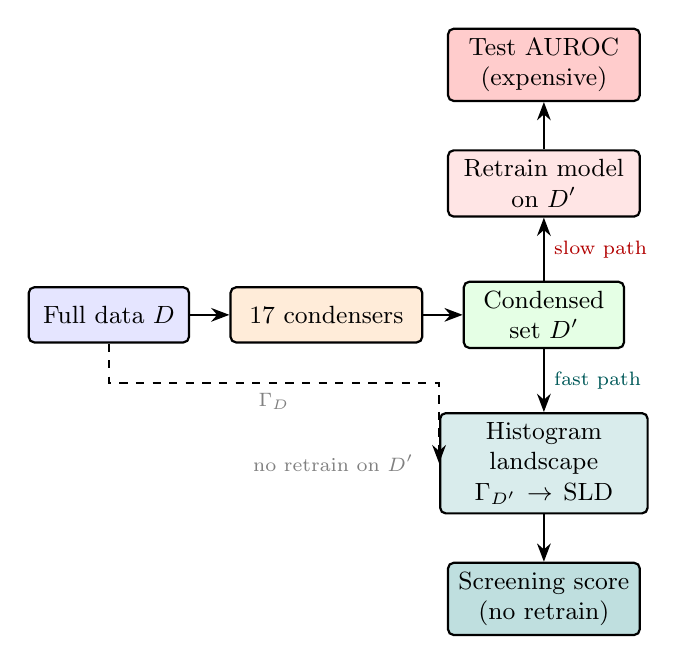
\begin{tikzpicture}[
  font=\small,
  node distance=4mm and 5mm,
  box/.style={rectangle, rounded corners=2pt, draw, thick,
              minimum height=7mm, text centered, fill=white},
  bigbox/.style={rectangle, rounded corners=2pt, draw=gray, thick,
                 fill=gray!8, inner sep=4pt},
  arr/.style={-Stealth, thick},
  dashed arr/.style={-Stealth, thick, dashed, gray},
]

% Full data
\node[box, fill=blue!10, text width=18mm] (fulldata) {Full data $D$};

% 17 condensers
\node[box, fill=orange!15, text width=22mm, right=of fulldata] (condensers)
  {17 condensers};

% Condensed set
\node[box, fill=green!10, text width=18mm, right=of condensers] (cset)
  {Condensed set $D'$};

% SLD path (no candidate retraining)
\node[box, fill=teal!15, text width=24mm,
      below=8mm of cset] (sld)
  {Histogram landscape\\$\Gamma_{D'} \to \mathrm{SLD}$};

% Verdict
\node[box, fill=teal!25, text width=22mm,
      below=6mm of sld] (verdict)
  {Screening score\\(no retrain)};

% Retrain path (expensive)
\node[box, fill=red!10, text width=22mm,
      above=8mm of cset] (retrain)
  {Retrain model\\on $D'$};

% Predictive-performance evaluation
\node[box, fill=red!20, text width=22mm,
      above=6mm of retrain] (acc)
  {Test AUROC\\(expensive)};

% Arrows
\draw[arr] (fulldata) -- (condensers);
\draw[arr] (condensers) -- (cset);
\draw[arr] (cset) -- (sld) node[midway, right, font=\scriptsize, teal!70!black]
  {fast path};
\draw[arr] (sld) -- (verdict);
\draw[arr] (cset) -- (retrain) node[midway, right, font=\scriptsize, red!70!black]
  {slow path};
\draw[arr] (retrain) -- (acc);

% Landscape feed from full data to SLD
\draw[arr, dashed] (fulldata.south) -- ++(0,-5mm) -|
  (sld.west) node[near start, below, font=\scriptsize, gray]
  {$\Gamma_D$};

% Label brace
\node[font=\scriptsize, gray, left=2mm of sld] {no retrain on $D'$};

\end{tikzpicture}
\caption{%
  \textbf{SLD evaluation pipeline.}
  After selecting a condensed set $D'$ from full data $D$ via any of 17
  condensers, the fast path computes the candidate's histogram split-gain
  landscape $\Gamma_{D'}$ under the same fixed prediction state as
  $\Gamma_D$. It provides a cheap screening signal before retraining on each
  candidate, in contrast to the slow path of retrain-and-test evaluation.%
}
\label{fig:pipeline}
\end{figure}

% ============================================================
%  SECTION 4: EXPERIMENTAL SETUP
% ============================================================

% 04_setup.tex  --  Experimental Setup

\section{Experimental Setup}
\label{sec:setup}

\subsection{Methods Evaluated}

We evaluate 17 condensation methods spanning five groups; \Cref{tab:methods}
gives the full taxonomy. \textbf{Geometry/classical coresets} include Random
sampling, Herding~\cite{welling2009herding}, and K-center~\cite{sener2018kcenter}.
\textbf{GBDT-native subsampling} methods include GOSS~\cite{ke2017lightgbm}
and MVS~\cite{ibragimov2019mvs}, adapted to produce static condensed sets.
\textbf{Gradient- and score-based selection} methods include GraNd,
EL2N~\cite{paul2021el2n}, CRAIG-style~\cite{mirzasoleiman2020craig},
GradMatch-style~\cite{killamsetty2021gradmatch}, and gradient sampling
(loss-weighted). \textbf{Distribution-matching distillation} is represented
by DistributionMatching~\cite{zhao2023dm} adapted to tabular features.
\textbf{Gain/landscape-based methods} form our primary family: HistDistill-Greedy
(the $(1-1/e)$-optimal coverage selector), HistDistill-Refined and
HistDistill-Density (controlled landscape-fidelity diagnostic baselines), gain
sketch, gain-path sketch, and the legacy gain-path refined method. The last
three are prior gain-path methods; the paper's main claim is the diagnostic and
benchmark, not a new state-of-the-art condenser. All adaptations produce static
surrogates: GOSS/MVS select the top scored instances under the fixed GBDT state;
GraNd, EL2N, CRAIG, and GradMatch use their published scoring or matching rules;
DistributionMatching runs on processed tabular features and shares full-data
bin edges for SLD scoring.
Short names follow the original methods: GOSS is Gradient-based One-Side
Sampling, MVS is Minimal Variance Sampling, GraNd is Gradient Normed, EL2N is
Error L2 Norm, CRAIG is a gradient-matching coreset method, DM abbreviates
DistributionMatching, and HD abbreviates HistDistill.

\subsection{Datasets and Protocol}

Our experiments use public tabular datasets drawn from
OpenML~\cite{vanschoren2013openml} and the Penn Machine Learning Benchmarks
(PMLB)~\cite{olson2017pmlb}; several entries originate from UCI-style benchmark
datasets. The full inventory appears in \Cref{tab:datasets}. The repository
lists the exact OpenML/PMLB identifiers and processed split checksums. The core
study is on binary classification. For each dataset we
condense the training set to five budgets, $\{10, 25, 50, 100, 200\}$ rows, and
repeat every (dataset, method, budget) configuration over five random seeds.
Across the 26 binary datasets and the five core methods this gives $3{,}250$
retrained-model evaluations for headline performance (\Cref{tab:headline}) and
$650$ landscape-fidelity measurements, one per dataset, method, and budget.

The broader 17-method analysis uses the same 26 datasets, budgets 25/50, and
three seeds, giving 156 cells per method for \Cref{fig:universal}. The
decomposition comparison (\cref{tab:decomp}) isolates the two reference-chain
failure modes; its absolute AUROCs are not compared to the pooled headline
values. Additional studies include the $1{,}872$-cell split-noise robustness
analysis, multiclass classification, regression, hyperparameter optimisation
(HPO) transfer, and a large-scale analysis on Covertype/SUSY/HIGGS with 400-row
condensed sets; \cref{sec:limits,sec:results-scale} give details.

\subsection{Metrics}

\textbf{Downstream performance.}
Binary classification: AUROC. Multiclass: one-vs-rest macro-AUROC.
Regression: $R^2$. All scores use the model retrained on the condensed set
and evaluated on the held-out test set.

\textbf{Landscape fidelity.}
The relative $\mathrm{SLD}_\infty$ is defined in \eqref{eq:sld}.
\Cref{fig:sldlaw} uses raw (un-normalised) $\ell_\infty$ error to show
scale confounding; raw values are not comparable across datasets.
Split-regret normalises the gain cost of following the surrogate's argmax
split over the full-data optimum. Let $g^* = [\Gamma_D]_{f^*,b^*}$ be the
full-data optimal gain, and $\hat{g} = [\Gamma_D]_{\hat{f},\hat{b}}$ the gain
of the surrogate's preferred split $(\hat{f},\hat{b})=\arg\max[\Gamma_{D'}]$:
\begin{equation}
\mathrm{regret}(D,D') = \max\!\left(0,\;\frac{g^* - \hat{g}}
                                              {\max(|g^*|,\varepsilon)}\right).
\label{eq:regret}
\end{equation}

\textbf{Error decomposition.}
Three models form a reference chain: the full-data model with AUROC $A_r$
(structure reference); the condensed-set tree with leaves refit on full data,
AUROC $A_\ell$; and the condensed-set model with its own leaves, AUROC $A_d$.
\begin{equation}
\epsilon_{\mathrm{struct}} = A_r - A_\ell,\qquad
\epsilon_{\mathrm{leaf}}   = A_\ell - A_d.
\label{eq:decomp}
\end{equation}
Leaf-population mismatch $\mathrm{pop}(D')=\|p^*-p_{D'}\|_1$ measures how
representatively $D'$ fills the model leaves, where $p^*$ and $p_{D'}$ are the
empirical leaf-occupancy distributions on $D$ and $D'$.

\subsection{Learners and Reproducibility}

The reference landscape and primary downstream learner use histogram XGBoost.
Robustness checks additionally use LightGBM, CatBoost/fallback histogram
boosting, random forests, and multilayer perceptrons (MLPs). All datasets are
public and preprocessing is deterministic: categorical features follow the
repository scripts, numerical features use shared full-data bin edges, and
splits use stratified seeds where labels permit. The repository (linked in the contributions) contains seeds, hyperparameters,
package versions, processed tables, and plotting code needed to reproduce all
reported results.


% ---- Table 1: Method taxonomy ----
\begin{table}[t]
\centering
\caption{The 17 condensation methods. $\dagger$: adapted from differentiable settings.}
\label{tab:methods}
\tiny
\setlength{\tabcolsep}{2pt}
\begin{tabular}{@{}llp{20mm}@{}}
\toprule
\textbf{Family} & \textbf{Method} & \textbf{Signal / citation} \\
\midrule
\multirow{3}{*}{Geometry}
  & Random         & Uniform \\
  & Herding        & Moments~\cite{welling2009herding} \\
  & K-center       & Coverage~\cite{sener2018kcenter} \\
\midrule
\multirow{2}{*}{GBDT-native}
  & GOSS$^\dagger$  & Grad-norm~\cite{ke2017lightgbm} \\
  & MVS$^\dagger$   & Min-var~\cite{ibragimov2019mvs} \\
\midrule
\multirow{5}{*}{Gradient}
  & GraNd$^\dagger$       & Norm at init~\cite{paul2021el2n} \\
  & EL2N$^\dagger$        & Error L2~\cite{paul2021el2n} \\
  & CRAIG$^\dagger$        & Submod.~\cite{mirzasoleiman2020craig} \\
  & GradMatch$^\dagger$   & Grad match~\cite{killamsetty2021gradmatch} \\
  & Grad.\ samp.$^\dagger$ & Loss-weighted \\
\midrule
Distrib.
  & DistributionMatching & Distr.\ match~\cite{zhao2023dm} \\
\midrule
\multirow{6}{*}{Gain / landscape}
  & HD-Greedy  & $(1-1/e)$ coverage \\
  & HD-Refined & Landscape fidelity \\
  & HD-Density & Land.+density \\
  & Gain sketch & Gain sketch \\
  & Gain-path sk. & Gain-path sketch \\
  & Legacy gp & Gain-path refined \\
\bottomrule
\end{tabular}
\end{table}

% ============================================================
%  SECTION 5: RESULTS
% ============================================================

% 05_results.tex  --  Results

\section{Results}
\label{sec:results}

\subsection{Does the Landscape Predict Performance?}
\label{sec:results-ordering}

Method-level split-regret ranks method families in the small-to-mid-size
benchmark (\Cref{fig:universal,tab:allmethods}). The score is computed before
candidate retraining and is strongly monotone with eventual AUROC at the
method-mean level: gain-path methods sit in the low-regret/high-AUROC corner,
while the coverage-optimal HD-Greedy method sits at the opposite extreme.
Gradient sampling is the main exception, and the decomposition below shows why:
its problem is leaf-value estimation, not split-structure preservation. This
17-method diagnostic grid uses 26 datasets, two audited budgets, and three
seeds, and is separate from the five-budget, five-seed core grid in
\Cref{tab:headline}. The large-scale audit in \cref{sec:results-scale} bounds
the claim: once high-gain margins are cleared on very large datasets, root
split-regret loses rank resolution.

% ---- Figure 2: Universal SLD map (headline) ----
\begin{figure}[!t]
\centering
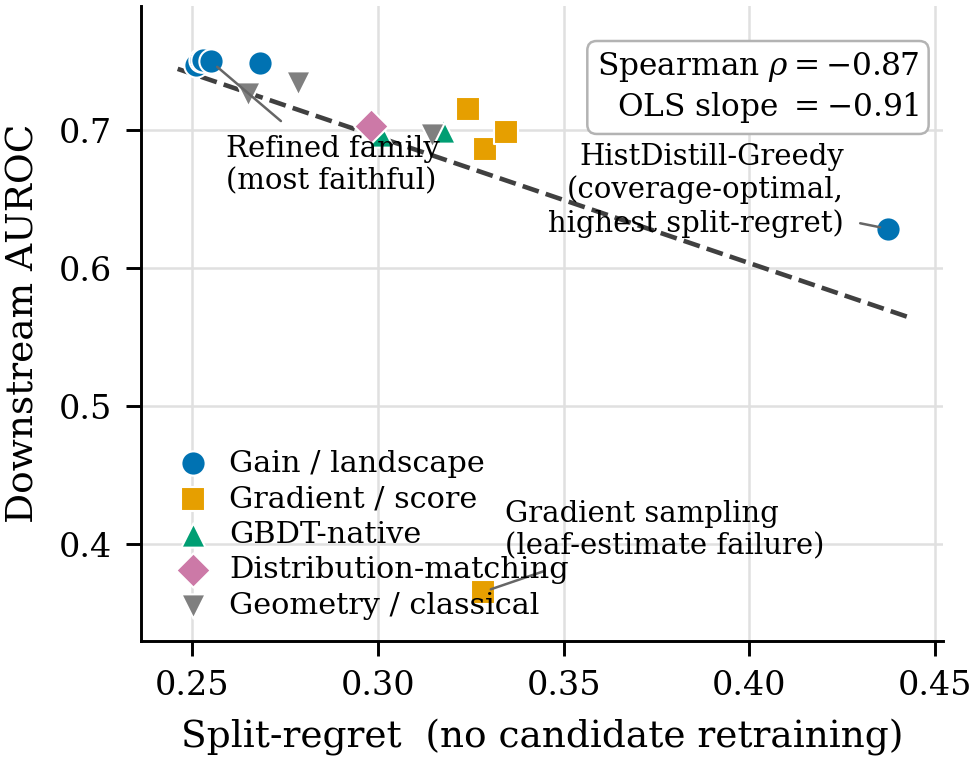
\includegraphics[width=\columnwidth]{figures/fig_c1_universal.png}
\caption{%
  \textbf{No-candidate-retraining method audit.}
  Each point is one condensation method. Lower split-regret, computed before
  candidate retraining, tracks higher downstream AUROC over 156
  dataset--budget--seed cells (Spearman $\rho=-0.87$, OLS slope $-0.91$).%
}
\label{fig:universal}
\end{figure}

% ---- Table 2: Headline performance + fidelity ----
\begin{table}[!t]
\centering
\caption{Headline performance and diagnostics for five core methods (3,250 cells).
AUROC uses mean$\pm$95\% CI over dataset clusters; avg.\ rank lower is better.
Raw SLD$_\infty$ is diagnostic only and is not a cross-dataset fidelity score;
speedup is relative to full-data retraining on the same dataset/learner.}
\label{tab:headline}
\scriptsize
\setlength{\tabcolsep}{3pt}
\begin{tabular}{@{}lcccc@{}}
\toprule
\textbf{Method} & \textbf{AUROC} & \textbf{Rank} &
  \textbf{Raw SLD}$_\infty$ \textbf{diag.} & \textbf{Speedup} \\
\midrule
Full data & $0.812 \pm 0.062$ & -- & -- & 1.0$\times$ \\
Legacy gain-path  & $0.743 \pm 0.057$ & 2.60 & 99.4  & 3.9$\times$ \\
HistDistill-Refined  & $0.742 \pm 0.057$ & 2.68 & 93.6 & 3.5$\times$ \\
HistDistill-Density  & $0.742 \pm 0.057$ & 2.65 & 93.7 & 3.5$\times$ \\
Herding           & $0.731 \pm 0.054$ & 3.44 & 174.1  & 3.8$\times$ \\
Random            & $0.724 \pm 0.056$ & 3.63 & 138.3  & 4.0$\times$ \\
\bottomrule
\end{tabular}
\end{table}

The gradient-sampling AUROC is an audited failure mode rather than a plotting
artifact: its deployed AUROC is also low in the reference-chain subset
(\Cref{tab:decomp}), where the error is leaf-estimate dominated. The
method-level association is not driven only by this point or by HD-Greedy:
excluding both leaves Spearman $\rho=-0.85$ over the remaining 15 methods.

% ---- Table 3: Universal 17-method audit ----
\begin{table}[!t]
\centering
\caption{Seventeen-method diagnostic audit. Values are method means
$\pm$95\% CI over dataset clusters, over 156 dataset--budget--seed cells.
Lower split-regret and higher AUROC are better. EL2N and GraNd coincide after
rounding under the fixed-state adaptation used here.}
\label{tab:allmethods}
\tiny
\setlength{\tabcolsep}{2.5pt}
\begin{tabular}{@{}lrr@{}}
\toprule
\textbf{Method} & \textbf{AUROC} & \textbf{Regret} \\
\midrule
Gain-path sketch & $0.748\pm0.062$ & $0.251\pm0.079$ \\
Legacy gain-path & $0.751\pm0.062$ & $0.252\pm0.079$ \\
HD-Density & $0.751\pm0.061$ & $0.253\pm0.073$ \\
HD-Refined & $0.750\pm0.062$ & $0.255\pm0.077$ \\
Random & $0.726\pm0.060$ & $0.265\pm0.064$ \\
Gain sketch & $0.749\pm0.062$ & $0.268\pm0.081$ \\
Herding & $0.734\pm0.059$ & $0.279\pm0.082$ \\
DM & $0.703\pm0.062$ & $0.298\pm0.075$ \\
MVS & $0.697\pm0.058$ & $0.301\pm0.068$ \\
K-center & $0.697\pm0.062$ & $0.315\pm0.079$ \\
GOSS & $0.700\pm0.058$ & $0.317\pm0.073$ \\
GradMatch & $0.715\pm0.057$ & $0.324\pm0.086$ \\
Grad.\ samp. & $0.366\pm0.067$ & $0.328\pm0.078$ \\
EL2N & $0.686\pm0.056$ & $0.329\pm0.071$ \\
GraNd & $0.686\pm0.056$ & $0.329\pm0.071$ \\
CRAIG & $0.699\pm0.061$ & $0.335\pm0.082$ \\
HD-Greedy & $0.629\pm0.050$ & $0.437\pm0.106$ \\
\bottomrule
\end{tabular}
\end{table}

Negative leaf gaps mean deployed condensed leaves slightly outperform the
full-data leaf refit under this diagnostic chain, usually through regularisation
or favourable condensed weighting.

Lower raw SLD predicts higher AUROC within a dataset, but pooling across
datasets is confounded (\Cref{fig:sldlaw}). Within each dataset, lower raw
$\delta_\infty$ corresponds to better retrained AUROC; after pooling datasets,
the trend can invert because dataset scale affects both raw SLD magnitude and
absolute AUROC. Raw SLD should therefore be used for within-dataset,
within-budget method comparison, not as a cross-dataset absolute score.

% ---- Figure 3: SLD law scatter ----
\begin{figure}[!t]
\centering
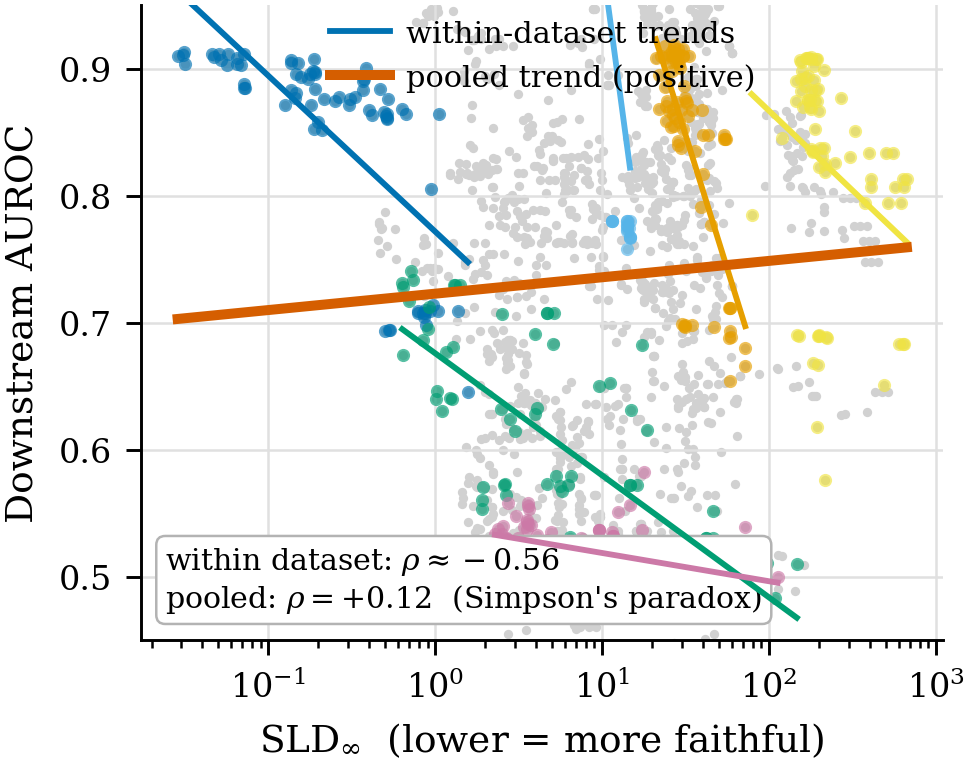
\includegraphics[width=\columnwidth]{figures/fig_c2_sldlaw.png}
\caption{%
  \textbf{Within-dataset SLD trend.}
  Coloured lines are within-dataset fits on log-scale raw SLD; the average
  within-dataset trend is negative. The pooled fit reverses because dataset
  scale confounds raw SLD and AUROC.%
}
\label{fig:sldlaw}
\end{figure}

\subsection{Coverage Is Not Predictive Fidelity}
\label{sec:results-coverage}

The near-optimal coverage selector is weak by downstream predictive
performance (\Cref{fig:coverage,tab:coverage}). HD-Greedy optimises
split-threshold coverage and achieves the expected coverage win, but this
objective is not the one that preserves downstream AUROC. The method lands in
the bottom tier of the 17-method audit (\Cref{tab:allmethods}); unweighted
threshold coverage and gain-weighted landscape fidelity are different
objectives.

% ---- Figure 4: Selector coverage ----
\begin{figure}[!t]
\centering
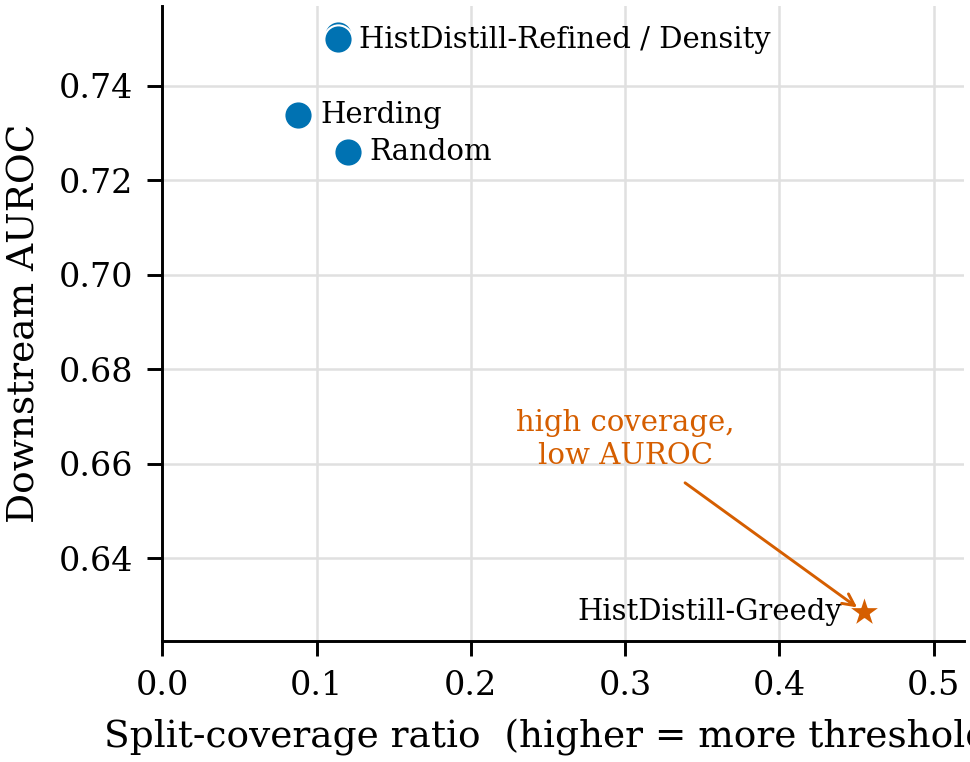
\includegraphics[width=\columnwidth]{figures/fig_c3_coverage.png}
\caption{%
  \textbf{Coverage is not predictive fidelity.}
  HD-Greedy covers the most high-gain split thresholds, but the accurate
  methods occupy a different region of the coverage--AUROC plane.%
}
\label{fig:coverage}
\end{figure}

% ---- Coverage paradox table ----
\begin{table}[!t]
\centering
\caption{Coverage metrics versus AUROC on the two-budget coverage audit.
Cov. is high-gain split coverage; Proxy is coverage divided by the proxy upper
bound.}
\label{tab:coverage}
\scriptsize
\setlength{\tabcolsep}{2pt}
\begin{tabular}{@{}lrrrrr@{}}
\toprule
\textbf{Method} & \textbf{Cov25} & \textbf{Proxy25} &
  \textbf{Cov50} & \textbf{Proxy50} & \textbf{AUROC} \\
\midrule
HD-Greedy & 0.371 & 1.000 & 0.539 & 1.000 & 0.629 \\
Random & 0.082 & 0.246 & 0.159 & 0.299 & 0.726 \\
HD-Refined & 0.075 & 0.223 & 0.152 & 0.286 & 0.750 \\
HD-Density & 0.075 & 0.223 & 0.152 & 0.286 & 0.751 \\
Herding & 0.059 & 0.183 & 0.118 & 0.229 & 0.734 \\
\bottomrule
\end{tabular}
\end{table}

The decomposition shows that the coverage failure is structural, whereas
gradient sampling fails for a different reason (\Cref{fig:decomp,tab:decomp}).
The reference chain separates structure error from leaf-estimate gap.
HD-Greedy's loss comes from choosing the wrong gain-weighted structure, not from
poor leaf values after its structure is fixed. Gradient sampling is the
opposite diagnostic case: its population mismatch is low, but its leaf-estimate
gap is high, pointing to distorted within-leaf gradient/Hessian or reweighting
statistics.

% ---- Figure 5: Error decomposition ----
\begin{figure}[!t]
\centering
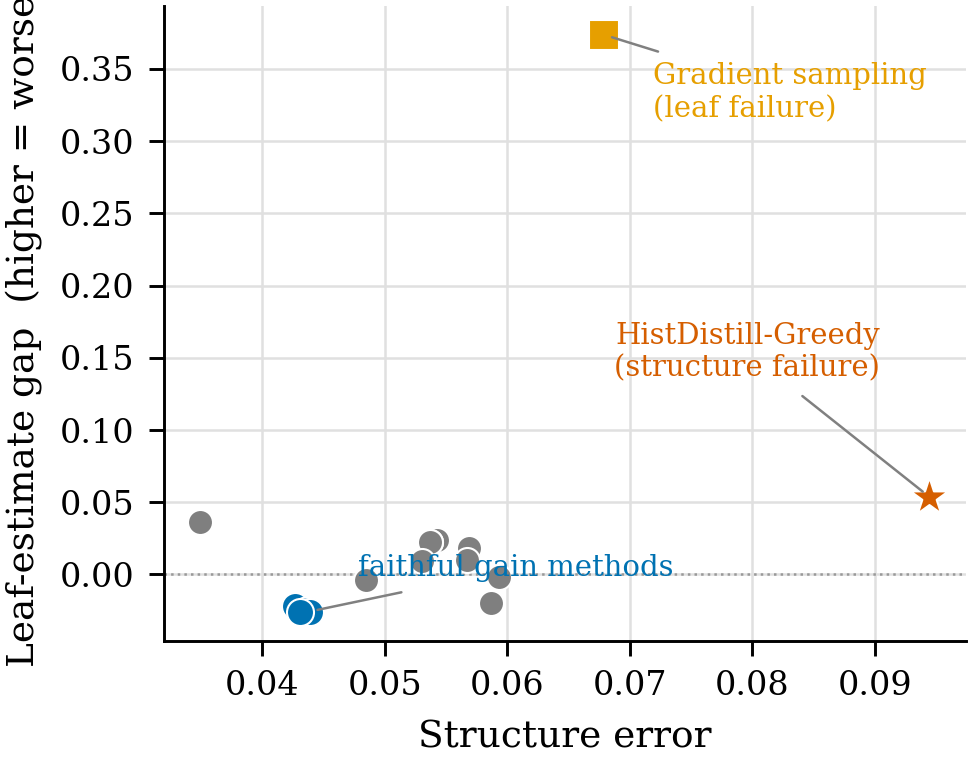
\includegraphics[width=\columnwidth]{figures/fig_c4_decomp.png}
\caption{%
  \textbf{Two failure modes.}
  HD-Greedy is structure-dominated; gradient sampling is leaf-estimate dominated.
  Faithful gain methods occupy the low-error corner.%
}
\label{fig:decomp}
\end{figure}

% ---- Decomposition table ----
\begin{table}[!t]
\centering
\caption{Error decomposition on the diagnostic subset used to illustrate both
failure modes. Absolute AUROCs differ from the pooled values in
\Cref{tab:headline,fig:universal}. Structure error is reference minus leaf-refit;
leaf gap is leaf-refit minus deployed.}
\label{tab:decomp}
\scriptsize
\setlength{\tabcolsep}{2.5pt}
\begin{tabular}{@{}lrrrrr@{}}
\toprule
\textbf{Method} & \textbf{Dep.} & \textbf{Leaf} &
  \textbf{Str.\ Err} & \textbf{Leaf Gap} & \textbf{Pop.} \\
\midrule
HD-Greedy     & 0.643 & 0.696 & 0.094 & 0.054 & 0.243 \\
Grad.\ samp.  & 0.349 & 0.723 & 0.068 & 0.374 & 0.133 \\
DM            & 0.720 & 0.756 & 0.035 & 0.036 & 0.235 \\
K-center      & 0.713 & 0.737 & 0.054 & 0.024 & 0.196 \\
MVS           & 0.724 & 0.734 & 0.057 & 0.010 & 0.088 \\
GradMatch     & 0.734 & 0.732 & 0.059 & $-0.002$ & 0.113 \\
HD-Refined    & 0.773 & 0.747 & 0.044 & $-0.026$ & 0.060 \\
Legacy gp     & 0.774 & 0.748 & 0.043 & $-0.026$ & 0.068 \\
\bottomrule
\multicolumn{6}{@{}l@{}}{\scriptsize Decomposition-subset anchors: full AUROC $=0.826$, reference $=0.791$.}
\end{tabular}
\end{table}

\subsection{How Much Can Structure Be Perturbed?}
\label{sec:results-dose}

Calibrated split-gain noise exposes a margin-linked robustness pattern for GBDT
structure (\Cref{fig:dose,tab:dose}). AUROC and split agreement stay flat while
the margin condition in \eqref{eq:prop1} holds; beyond that point, agreement
drops first and AUROC degrades mildly. The result explains why aggressive
condensation can work when the dominant split margins are preserved, and why
corrupting high-gain structure is disproportionately costly.

% ---- Figure 6: Dose response ----
\begin{figure}[!t]
\centering
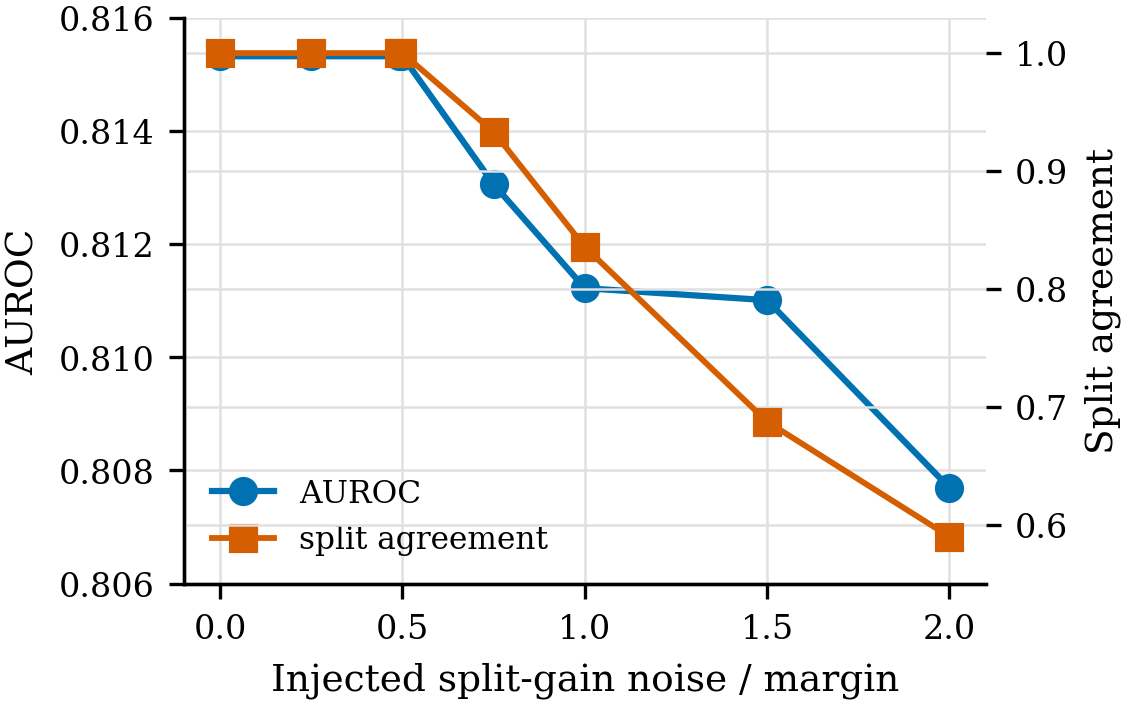
\includegraphics[width=\columnwidth]{figures/phase2_e18_downstream_dose_response.png}
\caption{%
  \textbf{Robustness pattern.}
  Split agreement drops after dose $0.5$; AUROC degrades mildly as calibrated
  split-gain noise exceeds the margin.%
}
\label{fig:dose}
\end{figure}

% ---- Dose response table ----
\begin{table}[!t]
\centering
\caption{Dose-response: 26 binary datasets, 1,872 cells. Values are
mean$\pm$95\% CI over dataset clusters; eight injected-noise levels are grouped
into five displayed rows.}
\label{tab:dose}
\scriptsize
\setlength{\tabcolsep}{3pt}
\begin{tabular}{@{}rcccc@{}}
\toprule
\textbf{Dose} & \textbf{AUROC} & \textbf{$\Delta$AUROC} &
  \textbf{Agree.} & \textbf{Regret} \\
\midrule
$\leq$0.50 & $0.815\pm0.068$ & 0.000 & $1.000\pm0.000$ & 0.000 \\
0.75 & $0.813\pm0.069$ & $-0.002$ & $0.933\pm0.002$ & 0.011 \\
1.00 & $0.811\pm0.069$ & $-0.004$ & $0.836\pm0.004$ & 0.030 \\
1.50 & $0.811\pm0.069$ & $-0.004$ & $0.687\pm0.008$ & 0.069 \\
2.00 & $0.808\pm0.070$ & $-0.008$ & $0.590\pm0.011$ & 0.101 \\
\bottomrule
\end{tabular}
\end{table}

\subsection{Performance, Fidelity, and Cost}
\label{sec:results-practical}

The top of the core grid is practically tied
(\Cref{tab:headline,tab:pairwise}). HistDistill-Refined and
HistDistill-Density match the legacy gain-path selector in AUROC while
achieving the lowest landscape discrepancy among the core methods. The
Refined-vs.-Legacy mean difference is operationally negligible and its
dataset-clustered confidence interval crosses zero. At the studied small-data
budgets, condensed retraining gives a median $3$--$4\times$ speedup, with
median condensed training under half a second in the recorded runs; SLD itself
costs one histogram pass.

\subsection{Does the Diagnostic Hold at Scale?}
\label{sec:results-scale}

\textbf{Scale audit: the cost payoff grows with $N$, while ordering is
dataset-dependent.}
A real large-data audit with 400-row condensed sets shows the payoff and the
limit of the diagnostic at deployment scale
(\Cref{fig:large-scale,tab:large-scale,tab:large-auroc}). Speedup rises from
single digits at $20$k rows to hundreds or thousands at million-row scale.
Random has the best large-$N$ AUROC point estimate on all three datasets, but
the three-dataset paired audit is underpowered (two-sided Wilcoxon $p=0.25$
vs.\ HD-Refined and HD-Density), so the practical reading is convergence among
reasonable condensers. This is the regime thesis: HD-Refined beats Random in
24/26 small-to-mid-size datasets (\Cref{tab:pairwise}), yet Random has the
largest point estimate on all three very large datasets
(\Cref{tab:large-auroc}).

HIGGS illustrates the same margin mechanism as \Cref{fig:sldlaw,fig:dose}:
several methods have zero root split-regret because the dominant root split is
saturated, so leaf estimates or deeper structure determine AUROC. Root-level
regret still rejects severe failures, but it cannot finely rank reasonable
surrogates once the top split margin is cleared.

\begin{figure}[!t]
\centering
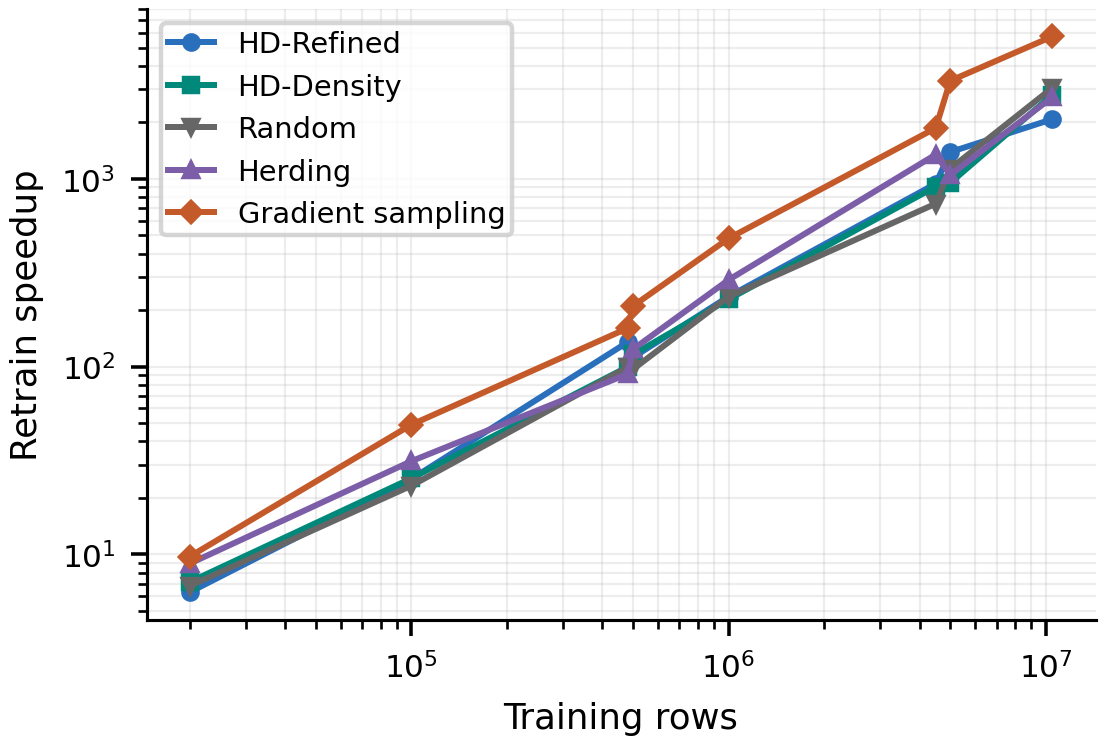
\includegraphics[width=\columnwidth]{figures/fig_large_scale_speedup.png}
\caption{%
  \textbf{Large-scale retraining payoff.}
  Log-log speedup for 400-row condensed retraining on Covertype, SUSY, and
  HIGGS. Points are single runs at observed dataset sizes, so no run-to-run CI
  is claimed for this scale audit.%
}
\label{fig:large-scale}
\end{figure}

\begin{table}[!t]
\centering
\caption{Large-scale audit at the largest training size per dataset. $\rho$ is
Spearman correlation over the five audited methods; negative $\rho$ means lower
split-regret aligns with higher AUROC. Each row is a single large-scale run.}
\label{tab:large-scale}
\scriptsize
\setlength{\tabcolsep}{3pt}
\begin{tabular}{@{}lrrr@{}}
\toprule
\textbf{Dataset} & \textbf{Rows} & $\boldsymbol{\rho}$ & \textbf{Top speedup} \\
\midrule
Covertype & 0.48M & $-0.36$ & $160\times$ \\
SUSY & 4.50M & $-0.97$ & $1{,}864\times$ \\
HIGGS & 10.50M & $0.11$ & $5{,}734\times$ \\
\bottomrule
\end{tabular}
\end{table}

\begin{table}[!t]
\centering
\caption{Large-scale AUROC at the largest training size. Full-data AUROCs are
0.897, 0.873, and 0.803 for Covertype, SUSY, and HIGGS. Random wins the
condensed point estimates, but the three-dataset paired audit is underpowered
($p=0.25$ against HD-Refined and HD-Density); no per-row CI is claimed because
the large-scale audit uses one full run per dataset/method.}
\label{tab:large-auroc}
\scriptsize
\setlength{\tabcolsep}{3pt}
\begin{tabular}{@{}lccc@{}}
\toprule
\textbf{Method} & \textbf{Cov.} & \textbf{SUSY} & \textbf{HIGGS} \\
\midrule
Full data & 0.897 & 0.873 & 0.803 \\
Random & \textbf{0.792} & \textbf{0.839} & \textbf{0.687} \\
HD-Refined & 0.747 & 0.818 & 0.648 \\
HD-Density & 0.781 & 0.794 & 0.641 \\
Herding & 0.719 & 0.780 & 0.450 \\
Grad.\ samp. & 0.377 & 0.219 & 0.364 \\
\bottomrule
\end{tabular}
\end{table}

\begin{figure}[!t]
\centering
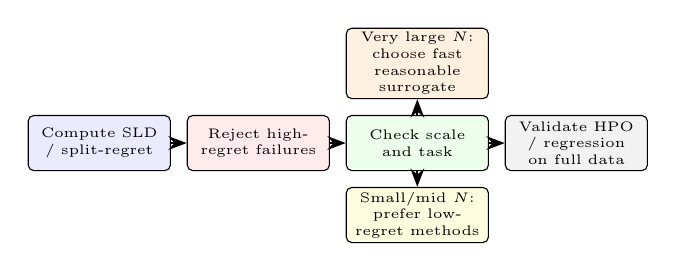
\begin{tikzpicture}[
  font=\tiny,
  node distance=2mm,
  box/.style={rectangle, rounded corners=2pt, draw, align=center,
              text width=17mm, minimum height=7mm, inner sep=1.5pt},
  arr/.style={-Stealth, thick}
]
\node[box, fill=blue!8] (sld) {Compute SLD / split-regret};
\node[box, fill=red!8, right=of sld] (reject) {Reject high-regret failures};
\node[box, fill=green!8, right=of reject] (size) {Check scale and task};
\node[box, fill=yellow!12, below=of size] (small) {Small/mid $N$: prefer low-regret methods};
\node[box, fill=orange!12, above=of size] (large) {Very large $N$: choose fast reasonable surrogate};
\node[box, fill=gray!10, right=of size] (validate) {Validate HPO / regression on full data};
\draw[arr] (sld) -- (reject);
\draw[arr] (reject) -- (size);
\draw[arr] (size) -- (small);
\draw[arr] (size) -- (large);
\draw[arr] (size) -- (validate);
\end{tikzpicture}
\caption{%
  \textbf{Operational workflow implied by the measurements.}
  SLD is most useful as a cheap screening diagnostic: reject high-regret
  failures, prefer low-regret methods only when margins are not saturated, and
  validate HPO, regression, and final deployment choices on full data.%
}
\label{fig:workflow}
\end{figure}

% ---- Pairwise tests for core methods ----
\begin{table}[!t]
\centering
\caption{Dataset-clustered core-method comparisons. $\Delta$ is the paired mean
AUROC difference over 650 dataset--budget--seed cells; confidence intervals
bootstrap the 26 dataset clusters.}
\label{tab:pairwise}
\scriptsize
\setlength{\tabcolsep}{2.5pt}
\begin{tabular}{@{}llrrr@{}}
\toprule
\textbf{Method} & \textbf{Comparator} & $\boldsymbol{\Delta}$ &
  \textbf{95\% CI} & \textbf{DS wins} \\
\midrule
HD-Refined & Legacy gp & $-0.00056$ & [$-0.0019$, $0.0008$] & 11/26 \\
HD-Density & Legacy gp & $-0.00056$ & [$-0.0016$, $0.0005$] & 9/26 \\
HD-Refined & Herding & 0.01183 & [$0.0037$, $0.0204$] & 18/26 \\
HD-Refined & Random & 0.01807 & [$0.0124$, $0.0233$] & 24/26 \\
\bottomrule
\end{tabular}
\end{table}


% ============================================================
%  SECTION 6: SCOPE AND LIMITATIONS
% ============================================================

% 06_limitations.tex  --  Where the Lens Stops

\section{Where the Lens Stops}
\label{sec:limits}

Three settings reveal the boundaries of what split-landscape fidelity can
predict. Each was identified by the diagnostic itself, not imposed externally.

\textbf{Regression: structure mismatch dominates and condensation cannot fix it.}
Across five regression datasets, deployed condensed models reach $R^2$ near
$0.16$--$0.17$, far below the full-data level of $0.63$. The reference-chain
decomposition attributes roughly three-quarters of the gap to tree-structure
mismatch and only one quarter to leaf-value errors. Refitting condensed-set
leaves on full data recovers part of the leaf gap but barely touches the
structure gap, and no method closes it at the budgets studied. SLD correctly
flags these surrogates as structurally unfaithful; it does not provide a fix.
Regression tasks require structure fidelity that small condensed sets cannot
deliver (\Cref{fig:regression}).

\begin{figure}[!t]
\centering
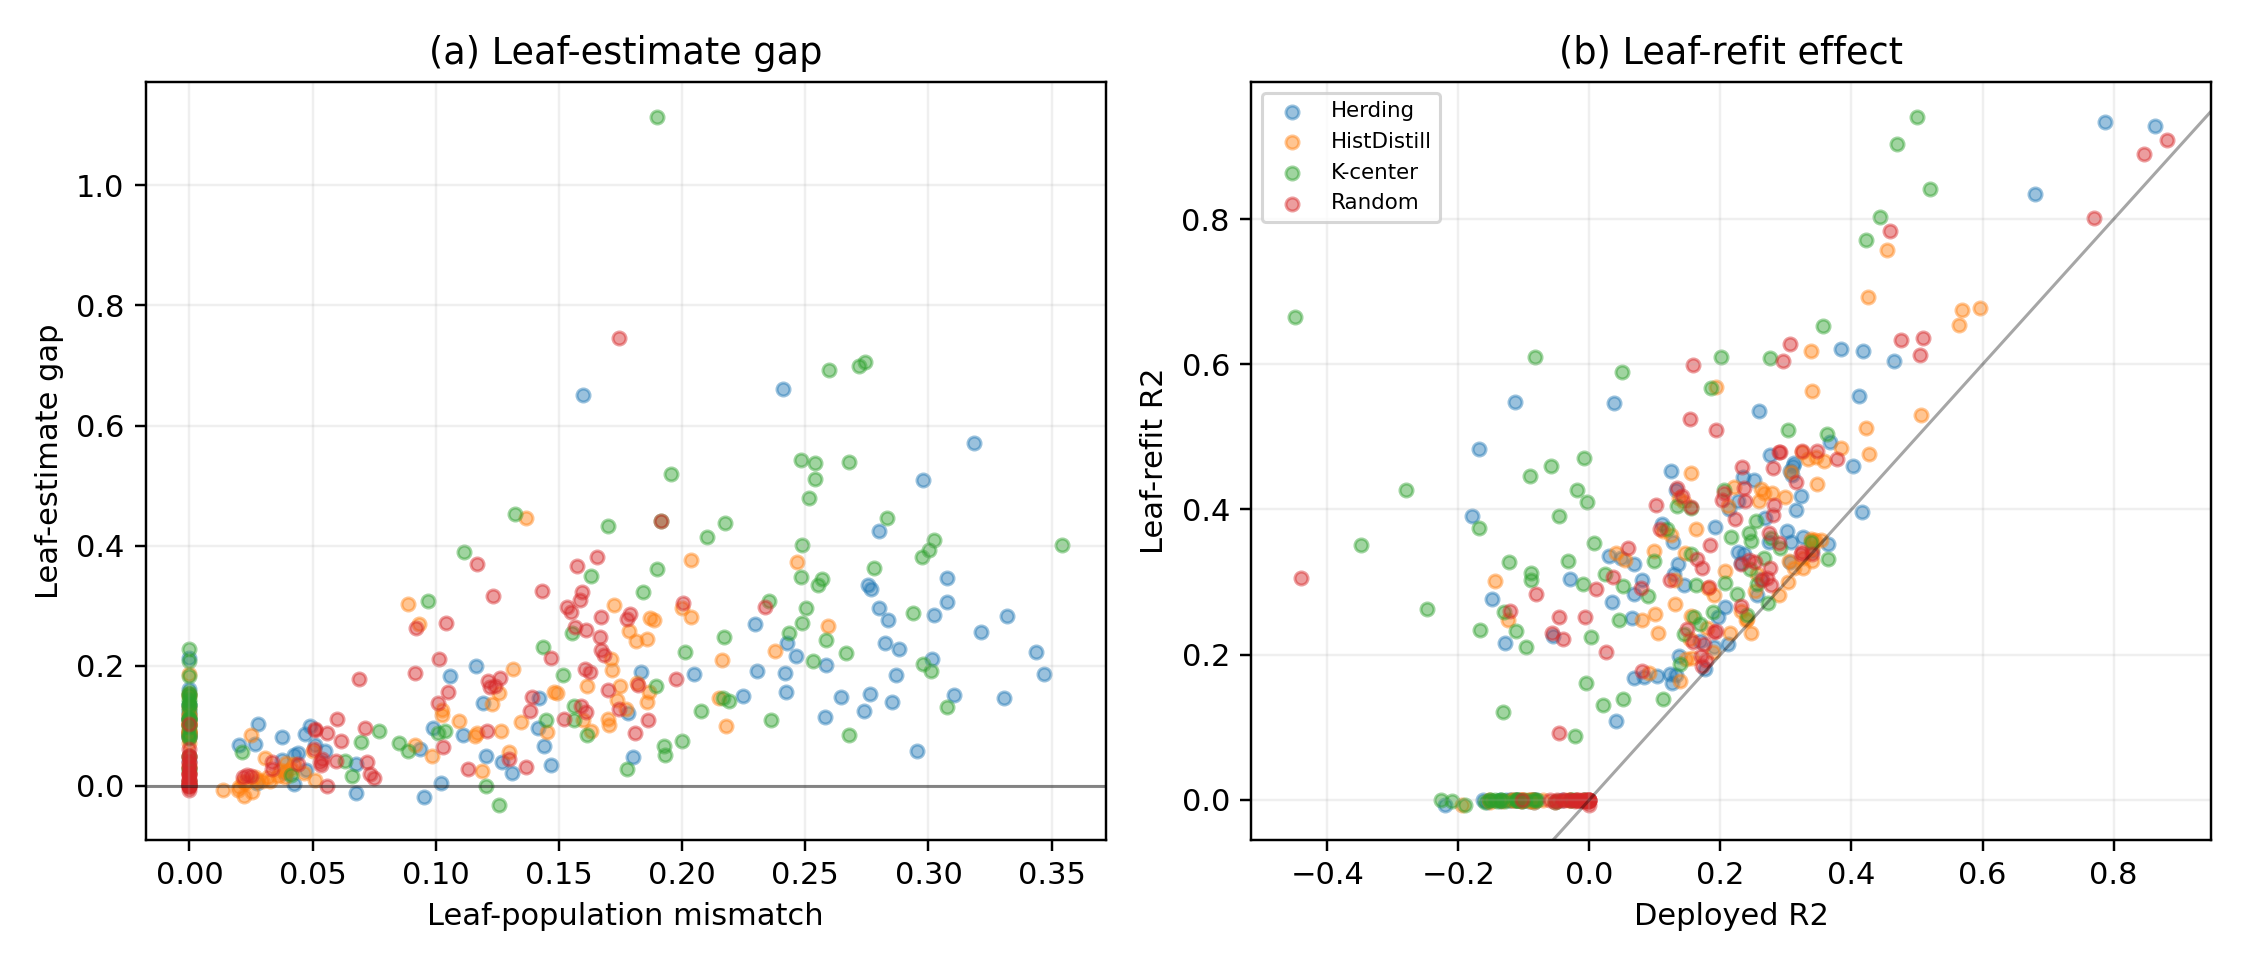
\includegraphics[width=\columnwidth]{figures/phase2_e21_regression_decomposition.png}
\caption{%
  \textbf{Regression decomposition.}
  Structure loss dominates for every method; leaf refitting helps modestly but
  does not close the gap to the structure reference.%
}
\label{fig:regression}
\end{figure}

\textbf{HPO configuration rankings transfer poorly from condensed to full data.}
Across 12 binary datasets, the top-3 agreement between condensed- and full-data
HPO rankings is $4.2\%$ and the top-1 match rate is $8.3\%$, with a
configuration rank correlation near zero ($0.15$). The median retraining
speedup is $1.6\times$, far too small to compensate. Condensed HPO can find a
competitive configuration by chance, but it finds a different one rather than
the full-data optimum. Top configurations selected on a condensed set should
always be validated on full data before deployment.

\textbf{Training-free selection of the single best method is unreliable.}
Split-regret reliably orders method families (Spearman $\rho=-0.87$), but
per-dataset selection of the single best method is harder. The top-3 success
rate of the SLD-based selector is $43.6\%$ and the top-1 rate is $12.2\%$
across all dataset--budget cells. When the second- and third-ranked methods are
close in regret, as is typical, the score is more useful as a rejection filter
for clearly poor surrogates than as an oracle.

Across five multiclass datasets the gain-path family improves over Random by
$1.3\%$ macro-AUROC, a positive but thin extension of the binary results. Taken
together, these findings confirm that SLD is a measurement instrument designed
around the GBDT split-gain objective; its signal erodes wherever that objective
does not govern the learning.


% ============================================================
%  SECTION 7: CONCLUSION
% ============================================================

% 07_conclusion.tex  --  Conclusion

\section{Conclusion}
\label{sec:conclusion}

We introduced the Split-Landscape Discrepancy, a no-candidate-retraining metric
that compares full-data and surrogate GBDT split-gain landscapes in one
histogram pass, and used it to study 17 condensation methods across 26 tabular
datasets. Method-level split-regret correlates with downstream AUROC at
Spearman $\rho=-0.87$, showing that the landscape comparison is a reliable
screening and family-ranking tool before any candidate is retrained.

The central finding overturns a natural intuition: a selector with a provable
$(1-1/e)$ coverage guarantee achieves the lowest downstream AUROC in the
study. Breadth of split-threshold coverage is not a proxy for predictive
fidelity, because downstream performance depends on preserving the
gain-weighted structure of the dominant splits, not on counting reproduced
thresholds. The reference-chain
decomposition (\cref{eq:decomp}) operationalises this distinction: coverage
failure is a structure failure, not a leaf failure, and each failure mode points
to a distinct debugging target, making the decomposition a practical debugging
tool.

The diagnostic reaches its limits at regression tasks, where structure mismatch
dominates and small condensed sets cannot overcome it; at HPO transfer, where
configuration rankings change even when final AUROC is similar; and at very
large scale, where dominant split margins saturate and the score becomes a
rejection filter rather than a fine-grained ranker. Within those boundaries,
the workflow is simple: compute split-regret to screen out poor candidates,
prefer low-regret methods when margins are not saturated, and validate
hyperparameter and regression decisions on full data. We release the benchmark
and implementation to support future evaluations of new condensation methods.


% Dataset inventory table (Appendix A) placed before bibliography so it
% floats into available space on the last body page.
\begin{table}[t]
\centering
\caption{Dataset inventory (binary; public via OpenML/PMLB).
$*$: focused binary suite.}
\label{tab:datasets}
\tiny
\setlength{\tabcolsep}{1.5pt}
\begin{tabular}{@{}lrr|lrr@{}}
\toprule
\textbf{Dataset} & \textbf{N} & \textbf{F} &
\textbf{Dataset} & \textbf{N} & \textbf{F} \\
\midrule
adult$^*$      & 20k & 14 & spambase$^*$  & 4{,}601 & 57 \\
australian$^*$ &  690 & 14 & agaricus      & 8{,}145 & 22 \\
bank\_mktg$^*$ & 20k & 16 & credit\_appr. &   690 & 15 \\
breast\_w$^*$  &  699 &  9 & electricity   & 20k &  8 \\
credit\_g$^*$  & 1k  & 20 & gametes (6)   & 1{,}600 & 20 \\
diabetes$^*$   &  768 &  8 & hill\_val.(2) & 1{,}212 & 100 \\
pc1$^*$        & 1{,}109 & 21 & kr\_vs\_kp & 3{,}196 & 36 \\
phoneme        & 5{,}404 &  5 & pc3, pc4   & $\sim$1{,}500 & 37 \\
qsar\_biodeg   & 1{,}055 & 41 & sick        & 3{,}772 & 29 \\
smoke          & 1{,}500 & 12 & tic\_tac    &   958 &  9 \\
\bottomrule
\end{tabular}
\end{table}

% ============================================================
%  BIBLIOGRAPHY
% ============================================================

\bibliographystyle{IEEEtran}
\bibliography{references}

\end{document}
